\begin{frame}
    \frametitle{異質變異數問題 heteroskedasticity}

    \begin{itemize}
        \item 當我的變異數隨 X 而改變
        \item 估計還是不偏且一致
        \item 但是估計值的標準誤差(SE)會有誤,導致檢定會出問題
    \end{itemize}
    \begin{figure}
        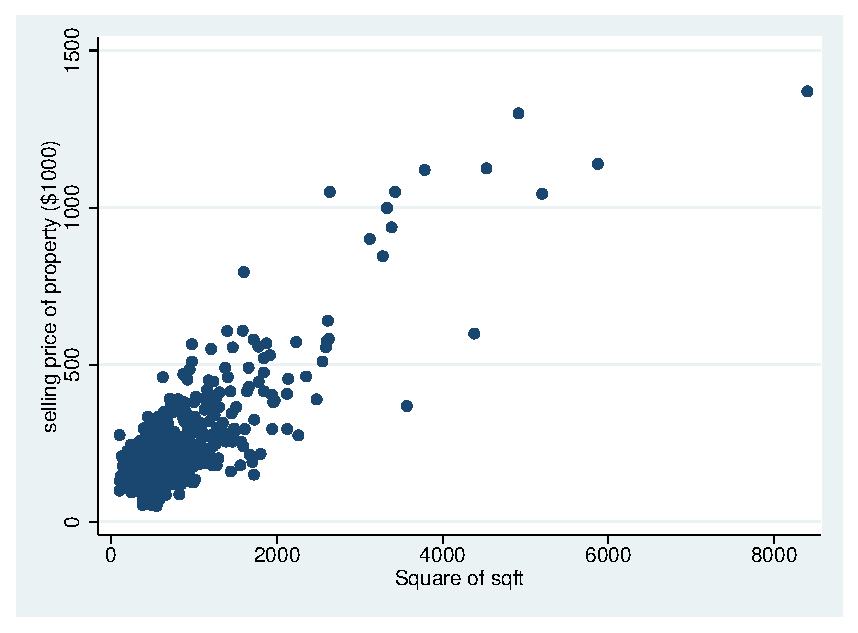
\includegraphics[width=0.8\textwidth]{figure/Heter_smaple.eps}
    \end{figure}
\end{frame}

\begin{frame}
    \frametitle{哪裡出問題?}
    \begin{itemize}
        \item 假設誤差項 $e_i$ 的變異數同為 $\sigma^2$ 之下,估計值 $\hat{\beta}_2$的變異數為
        \begin{equation}
            \operatorname{var}(\hat{\beta}_2 \given \mathbf{x}) = \frac{\sigma^2}{\sum_{i=1}^N (x_i - \bar{x})^2}
            =\sigma^2 (X'X)^{-1}
            \tag{8.6}
        \end{equation}
        \item 但實際上每一筆資料的誤差項,變異數不一樣,為 $\sigma_i^2$,用上面的就錯了,因為$\beta_2$的變異數這時會變成
        \begin{equation}
            \operatorname{var}(\hat{\beta}_2 \given \mathbf{x})=
            \left[
                \sum_{i=1}^N(x_i - \bar{x})
            \right]^{-1}
            \left[
                \sum_{i=1}^N(x_i - \bar{x})\sigma_i^2
            \right]
            \left[
                \sum_{i=1}^N(x_i - \bar{x})
            \right]^{-1}
            \tag{8.8}
        \end{equation}
    \end{itemize}
\end{frame}

\begin{frame}
    \frametitle{解決方法}
    \begin{enumerate}
        \item 既然在有異質變異數之下用OLS,估計值的變異數長這麼醜:
        \begin{equation*}
            \operatorname{var}(\hat{\beta}_2 \given \mathbf{x})=
            \left[
                \sum_{i=1}^N(x_i - \bar{x})
            \right]^{-1}
            \left[
                \sum_{i=1}^N(x_i - \bar{x})\sigma_i^2
            \right]
            \left[
                \sum_{i=1}^N(x_i - \bar{x})
            \right]^{-1}
        \end{equation*}
        那我乾脆就把上面的算出來吧:異質性穩健標準誤差(heteroskedasticity-robust standard errors, HR) 
        \vfill
        \item 既然知道這樣會有異質變異數問題,那不然我改變一下資料,把變異數變成一樣不就好了:廣義最小平方法
        \footnote{課本翻成「一般化最小平方法」,但他們怎麼會覺得一般化(GLS)跟普通(OLS)一般人分辨得出來?...}
    \end{enumerate}
\end{frame}

\begin{frame}
    \frametitle{檢測的方法}

    \begin{enumerate}
        \item 分兩種,看他們的殘差項發散程度一不一樣 --- GQ test
            \\ 檢定「醜人多作怪」
        \item 懷疑殘差項跟S個 X 有關連,就拿殘差跟那些回歸
            \begin{itemize}
                \item $NR^2 \sim \chi^2(S)$ --- NR2 test 
                \item 聯合檢定殘差回歸的係數 --- F test 
            \end{itemize}
        \item 將所有變數、變數的平方、交乘項,全部納入回歸 --- White Test
    \end{enumerate}

\end{frame}